\section{Data Pipeline}\label{sec:data-pipeline}
Aggregating and visualizing a decade of Citi Bike trip data introduces several challenges:
\begin{itemize}
    \item \textbf{Scale:} Hundreds of millions of trip records must be filtered and aggregated fast enough to keep the dashboard interactive.
    \item \textbf{Format Shifts:} Multiple data sources follow different packaging and column conventions, which have to be reconciled into a single schema.
    \item \textbf{Data Quality:} Each source carries missing values, outliers, and coverage gaps that would otherwise surface as misleading visuals.
\end{itemize}
Our pipeline addresses these challenges, enabling us to fulfill the core objectives outlined in our \proposalref{project proposal}.

\subsection{Pipeline Overview}
The pipeline turns raw sources into dashboard-ready data through three sequential stages, illustrated in Figure~\ref{fig:pipeline-overview}:
\begin{enumerate}
    \item \textbf{Data Acquisition} gathers the static datasets evaluated in our \technicalreportref{technical report}: the trip archives, hourly weather, bike-route geometries, and a station metadata snapshot.
    Each download is cached on disk with a freshness window, so repeated runs re-fetch only what has aged.

    \item \textbf{Cleaning and Normalization} leverages \emph{Polars} to unify heterogeneous source schemas, filter invalid records, and enrich each trip with key filter dimensions: date, hour, and day of the week.
    The pipeline then exports the cleaned data as compressed, monthly-partitioned \emph{Parquet} files.

    \item \textbf{Precomputation} aggregates cleaned trips into compact hourly and monthly summaries stored in \emph{PostgreSQL}.
    These include hourly ridership trends, station-level turnover, and station-pair trajectories, alongside synchronized hourly weather metrics to contextualize usage.
    Because monthly releases must be merged into these summaries without corrupting past runs, we write every table via dimension-keyed upserts, ensuring idempotent reloads and safe pipeline retries.
\end{enumerate}

In line with our project proposal, a \emph{GitHub Action} executes this complete sequence monthly and \textbf{publishes} the updated \emph{Docker} image to a public repository, keeping the dashboard continuously up to date.
\begin{figure}[htbp]
    \centering
    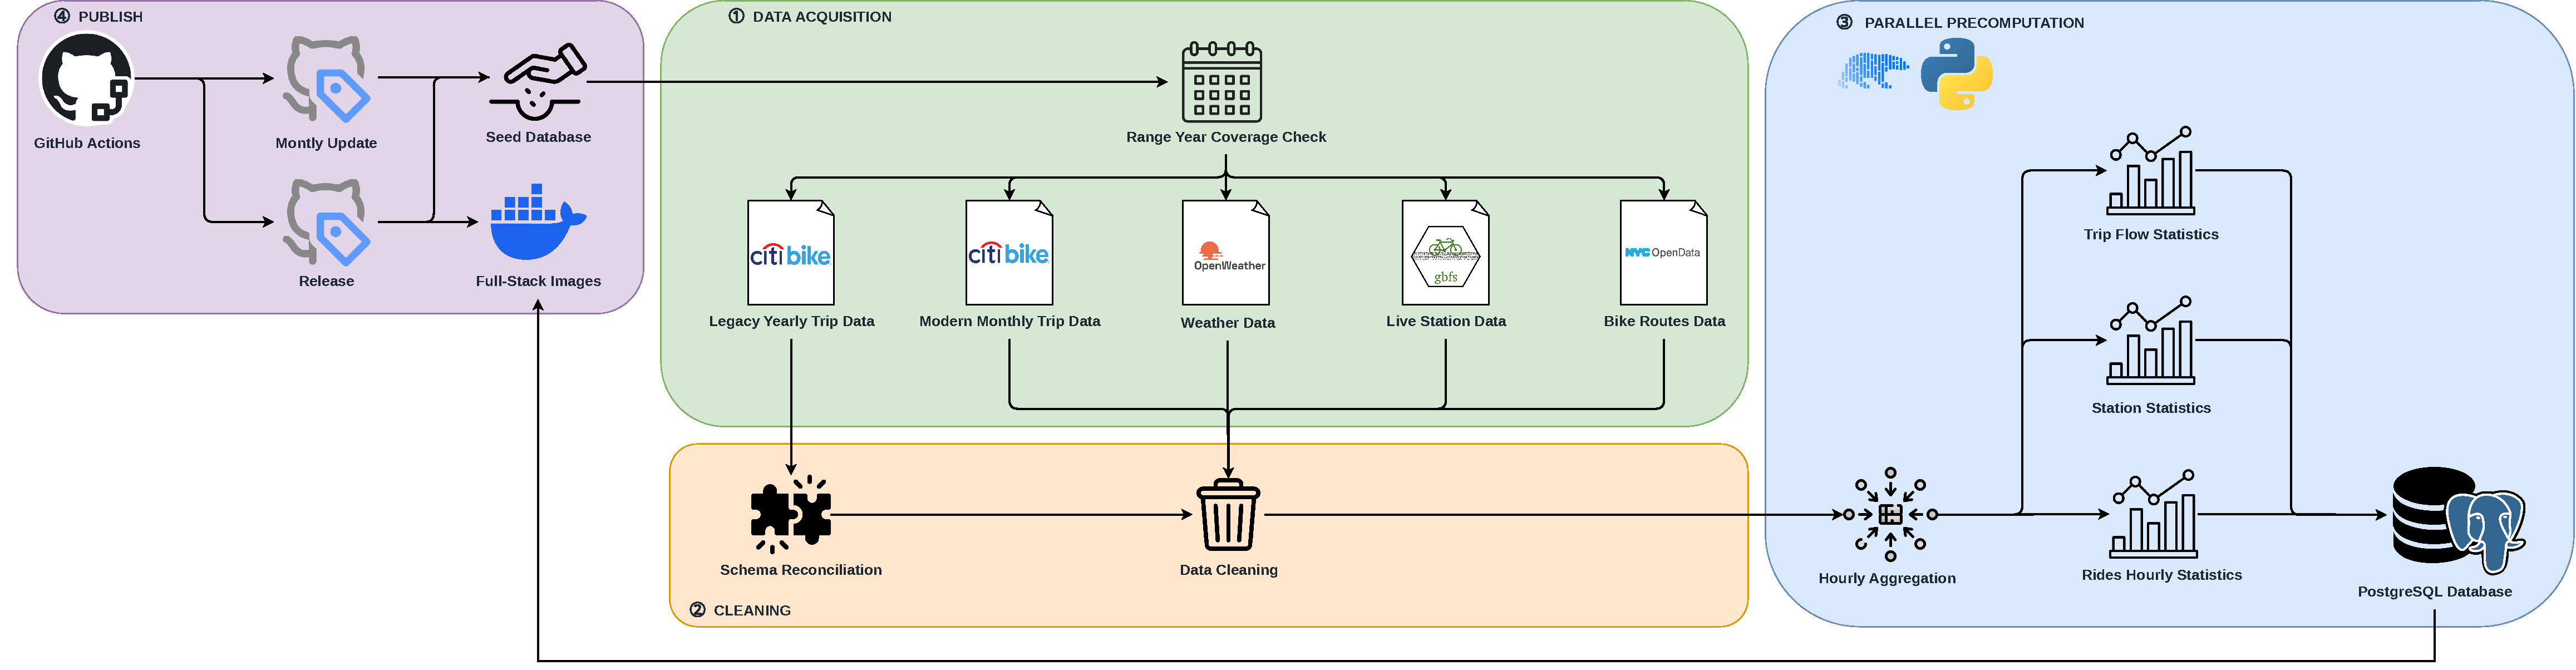
\includegraphics[width=\textwidth]{../media/report/data_pipeline.pdf}
    \caption{Data pipeline: the end-to-end architecture.}
    \label{fig:pipeline-overview}
\end{figure}

\subsection{Data Acquisition}
Of the four datasets gathered in this stage, the trip archives dominate: a decade of rides spans hundreds of millions of records, while the hourly weather, bike-route, and station metadata sources each arrive as a single, comparatively small file or API response.
To keep this asymmetry from exhausting standard hardware memory resources, the pipeline processes the trip archives through the following steps:
\begin{enumerate}
    \item \textbf{Streamed Downloading:} Downloads each archive to a temporary file in small chunks.
    \item \textbf{Monthly Processing:} Converts the data to a \emph{Parquet} file one month at a time.
    \item \textbf{Immediate Cleanup:} Deletes each intermediate file after loading.
\end{enumerate}
To accelerate this process, downloads overlap with database ingestion while worker threads compute aggregates in parallel.

To handle monthly releases without reprocessing the entire archive, the system tracks existing coverage and automatically expands requested ranges.
This guarantees a contiguous timeline while keeping each update proportional to the new data alone.

\subsection{Cleaning and Normalization}
Raw trip records inherit the data quality issues identified in our technical report, from missing fields and format drift to statistical outliers.

\paragraph{Missing Values}
Any records missing station, timestamp, user, or bike type data are immediately discarded.
Because the affected volume is negligible, discarding these rows preserves data integrity.

\paragraph{Legacy Schema Reformatting}
Beyond missing fields, format itself drifted over the years: Citi Bike archives arrive in two packaging formats, yearly bundles containing monthly archives (legacy), and flat monthly files (modern).
The pipeline automatically handles both structures, emitting a single data frame per month.

We reconcile these schema variations by retaining only the intersection of columns, discarding any fields not present across all years.

\paragraph{Trip Outliers}
Once records share a common schema, outliers remain the last distortion to filter out.
Three filters prevent extreme or invalid records from distorting duration and distance metrics:
\begin{itemize}
    \item \textbf{Negative Durations:} Records with timestamps where the end precedes the start are discarded.
    \item \textbf{Round Trips:} Rides sharing the same origin and destination are removed, as their zero straight-line distance would artificially affect distance averages.
    \item \textbf{Upper-Tail Extremes:} Long-duration and long-distance outliers are removed using a $95\%$ z-score threshold, calculated per month for each metric.
    Using a hard threshold would have been too aggressive, as the distribution could vary significantly across months and years.
\end{itemize}

\subsection{Precomputation}
Turning cleaned trip rows into dashboard-ready aggregates meant first establishing a complete time base, then keeping every query fast.

\paragraph{Time and Weather Spine}
To accurately calculate hourly utilization rates, the total number of elapsed hours within a given timeframe must be established.
Our initial design derived time buckets directly from the trip logs, operating on the assumption that at least one ride occurred per hour.
However, hours with zero activity, frequently corresponding with adverse weather conditions, were omitted, obscuring quiet periods.
To resolve this, we generated an independent, continuous hourly calendar spine and joined the trip data to it.

Similar to the time spine, visualizing ridership against weather conditions necessitates a two-dimensional grid.
Each hour of the spine is labelled with its observed weather condition, and hours without rides contribute zero-valued rows.
This yields a complete, rectangular dataset that renders reliably without requiring complex visualization workarounds.

\paragraph{Precomputing Statistics}
With a complete hourly base in place, the remaining challenge was speed.
Our initial design relied on \emph{Polars} to directly query raw \emph{Parquet} files without a database layer.
However, every user interaction triggered expensive full-table scans across hundreds of millions of raw rows, leading to unacceptable latency.

We shifted the heavy computational load to the ingestion pipeline by precomputing data at a one-hour granularity.
Because this granularity matches the finest detail required by the dashboard, we eliminate the need for on-the-fly full-table scans.

Not every query requires fine detail: a citywide yearly total needs only monthly sums, whereas a full hour-by-day-of-week breakdown is rarely used.
Scanning the finest hourly table for these coarser requests wastes compute proportional to the gap between required and available resolutions.
To keep query costs proportional to the resolution needed, three additional variants are rolled up alongside the hourly table: by month, hour of day, and day of week. 
Each variant is aggregated from the same cleaned trips to ensure consistency across all four.
Then, the backend routes each request to the smallest table able to answer it (Section~\ref{sec:backend}).